\documentclass[runningheads]{llncs}

\usepackage[T1]{fontenc}
\usepackage{graphicx}
\usepackage{algorithm2e}
\usepackage{booktabs}
\usepackage{amsmath,amssymb}
\usepackage{hyperref}

\begin{document}

\title{WiSARD F4RM: Feature-Restricted Round-Robin Random Mapping}

%\titlerunning{Abbreviated paper title}

\author{Anonymous Author(s)}

\authorrunning{Anonymous}

\institute{Affiliation anonymized for double-blind review}

\maketitle

\begin{abstract}
WiSARD's bit-to-RAM mapping has been left as a uniformly random permutation for four decades of research, treated as unexamined scaffolding. We show that this default leaves measurable accuracy on the table whenever the input has exploitable structure --- as thermometer-encoded continuous features do, owing to the monotonic redundancy between the $t$ bits of each encoded feature. We introduce F4RM (Feature-Restricted Round-Robin Random Mapping), a rule that constrains the mapping so every RAM reads from the maximum possible number of distinct input features, eliminating same-feature redundancy at zero cost: no new parameters, no change to training or inference, no additional hyperparameters beyond those of standard WiSARD. We extend F4RM to F4RMS (F4RM enSemble), which trains $K$ independently-seeded F4RM WiSARDs and aggregates their responses by summation. On 21 tabular classification datasets with 200 paired evaluations per dataset and Bonferroni-corrected significance, F4RM beats random mapping on 14 of 21 datasets and never significantly loses; F4RMS beats random mapping on 20 of 21 datasets and beats single F4RM on 19 of 21. We identify three data regimes --- dense-signal, redundant-feature, and small-sample --- that predict where each method helps, and provide a combinatorial account relating F4RM's benefit to feature independence in the input.

\keywords{Weightless neural networks \and WiSARD \and Feature encoding \and Ensemble methods \and Tabular classification}
\end{abstract}


\section{Introduction}
\label{sec:introduction}

Machine learning at the edge has renewed interest in architectures that trade small amounts of accuracy for large reductions in training cost, inference latency, and energy use. \emph{Weightless neural networks} (WNNs) are a distinctive option: they classify entirely through bit-addressed table lookups, with no weights, no backpropagation, and no floating-point arithmetic at inference. A WNN trains in a single pass and classifies with a handful of memory reads, and recent memory-efficient variants~\cite{susskind2022bthowen,susskind2023uleen,bacellar2022logicwisard} fit on milliwatt-scale hardware.

The canonical WNN architecture is WiSARD~\cite{aleksander1984wisard}, introduced in 1984 and studied extensively since then. WiSARD partitions a binary input vector into disjoint chunks, routes each to a RAM-based lookup table, and trains by incrementing the counter addressed by each chunk's bit pattern. The assignment of input bits to RAM positions --- the \emph{mapping} --- is fixed at initialization and shared across classes. In every standard implementation, this mapping is a uniformly random permutation.

The random mapping is an unexamined convention. Forty years of WiSARD research have explored bleaching~\cite{grieco2010producing}, ensemble structure~\cite{susskind2023uleen}, memory optimization~\cite{santiago2020bloom,bacellar2022logicwisard}, and most recently learnable mappings~\cite{bacellar2024dwn}, but the simple non-learned choice of \emph{which} bits go to \emph{which} RAM has, to the best of our knowledge, never been systematically studied. Randomness seems neutral: any permutation is valid, no design bias is introduced, and structure-agnosticism is appealing when the input has no privileged axis. These arguments are sound for genuinely structureless inputs like raw binary images, but they fail silently when WiSARD processes continuous features through \emph{thermometer encoding}~\cite{lima2020distributive}---a now-common preprocessing step that expands each feature into a monotonic block of bits.

The $t$ bits from a single thermometer-encoded feature are not independent: they encode only $t+1$ distinct patterns rather than $2^t$. When random mapping places multiple bits from the same feature into the same RAM, that RAM wastes address slots on redundant information while another RAM loses the chance to see that feature---a cost invisible per-RAM but consistent in aggregate.

We introduce \textbf{F4RM} (Feature-Restricted Round-Robin Random Mapping), a rule that constrains the mapping so each RAM reads from the maximum possible number of distinct features, while preserving random selection of \emph{which} thermometer level contributes. F4RM adds no parameters, no training cost, and runs once at initialization. We then extend it to \textbf{F4RMS} (F4RM enSemble), training $K$ independently-seeded F4RM WiSARDs and aggregating by summation---inheriting WiSARD ensembling practice~\cite{susskind2023uleen} while compounding F4RM's per-model benefit.

Our main contributions are fourfold. \textbf{(1) F4RM}, a feature-restricted round-robin mapping rule for WiSARD that maximizes per-RAM feature coverage at zero cost---no new parameters, no training or inference overhead, no hyperparameters beyond standard WiSARD. \textbf{(2) A mechanistic justification} based on the redundancy structure of thermometer encoding, identifying two independent costs of random mapping (feature-coverage loss and effective-capacity loss) and yielding a falsifiable prediction---that F4RM's benefit diminishes as model capacity grows---which we confirm empirically. \textbf{(3) F4RMS}, an ensemble of $K$ seeded F4RM WiSARDs with sum-of-response aggregation, inheriting established WiSARD ensembling practice while compounding F4RM's per-model benefit. \textbf{(4) Empirical validation} on 21 tabular classification datasets with 200 paired evaluations per dataset and Bonferroni-corrected significance: F4RM beats random mapping on 14 of 21 datasets and never significantly loses; F4RMS beats random mapping on 20 of 21 and beats single F4RM on 19 of 21.

The paper is divided as follows: Section~\ref{sec:related} positions our work against prior research on WiSARD mappings, memory optimizations, and weightless-network ensembles; Section~\ref{sec:f4rm} defines F4RM and its mechanistic justification; Section~\ref{sec:f4rms} extends it to the F4RMS ensemble. Sections~\ref{sec:methodology}--\ref{sec:results} describe the experimental setup and report results across 21 datasets, followed by limitations and conclusions.


\section{Related Work}
\label{sec:related}

We position F4RM against prior mapping strategies (Section~\ref{sec:related-mapping}), memory optimizations (Section~\ref{sec:related-memory}), and weightless-network ensembles (Section~\ref{sec:related-ensemble}).

\subsection{Mapping Strategies in WiSARD}
\label{sec:related-mapping}

The original WiSARD~\cite{aleksander1984wisard} uses a uniformly random bit-to-RAM mapping, and this has remained the default. Random mapping introduces no design bias and assumes no input structure---desirable for genuinely structureless inputs but wasteful, as Section~\ref{sec:limitation} argues, for thermometer-encoded continuous features.

BTHOWeN~\cite{susskind2022bthowen} replaces random mapping with a deterministic hash-based routing motivated by memory efficiency: hash collisions compress RAM state via a Bloom filter. The mapping remains randomness-based at heart---the hash is chosen for its collision distribution, not for structural awareness of the input. Differentiable WiSARD (DWN)~\cite{bacellar2024dwn} instead makes the mapping a learnable parameter via a differentiable relaxation, achieving strong accuracy gains but abandoning WiSARD's single-pass training simplicity. F4RM targets a different point: accuracy improvement at zero training cost and zero deviation from classical WiSARD training---the first WiSARD mapping rule that is structured but not learned.

\subsection{Memory and Architecture Optimizations}
\label{sec:related-memory}

A parallel line of work optimizes WiSARD's memory footprint and hardware efficiency without changing the core mapping principle. Bloom WiSARD~\cite{santiago2020bloom} replaces RAM lookup tables with Bloom filters, trading a small false-positive rate for substantial memory savings. ULEEN~\cite{susskind2023uleen} combines Bloom-filter storage with multi-submodel ensembles and Gaussian thermometer encoding for edge-inference deployments. LogicWiSARD~\cite{bacellar2022logicwisard} compiles trained WiSARD RAMs into logic functions, eliminating memory at inference time entirely.

These techniques are orthogonal to F4RM: they modify \emph{how} RAM state is stored or queried, not \emph{which} bits are assigned to which RAMs. A WiSARD using Bloom-filter RAMs can be F4RM-mapped with no modification to the Bloom filter apparatus. This complementarity is deliberate---restricting our contribution to the mapping rule alone lets F4RM slot into existing WiSARD pipelines without architectural changes.

\subsection{Ensemble Methods for Weightless Networks}
\label{sec:related-ensemble}

Ensembling weightless networks has been explored primarily as a route to reducing per-model memory while maintaining accuracy. ULEEN's multi-submodel architecture~\cite{susskind2023uleen} trains several smaller WiSARDs with different random permutations and aggregates their responses via summation---the same aggregation rule F4RMS adopts. ClusWiSARD~\cite{cardoso2017clus} uses a clustering-based ensemble motivated by intra-class heterogeneity rather than ensemble decorrelation.

The Random Subspace Method~\cite{ho1998random} is the natural starting point for any ensemble seeking decorrelation via input-view diversity. We found it unsuitable for WiSARD---subsets weaken each member faster than decorrelation recovers---so F4RMS instead derives diversity from the mapping randomness F4RM preserves, keeping each member at full F4RM strength.

Taken together, the prior literature leaves an unoccupied niche that F4RM targets directly: a mapping rule that is (i) structured rather than random, (ii) justified by the redundancy of the input encoding rather than by memory or hardware concerns, (iii) compatible with standard WiSARD training and existing memory optimizations, and (iv) extendable to an ensemble that reuses --- rather than replaces --- established aggregation practice. The remainder of this paper occupies that niche.


\section{F4RM: Feature-Restricted Round-Robin Random Mapping}
\label{sec:f4rm}

We cover background (Section~\ref{sec:preliminaries}), the cost of random mapping (Section~\ref{sec:limitation}), the F4RM rule and algorithm (Section~\ref{sec:f4rm-rule}), a testable prediction (Section~\ref{sec:testable-prediction}), and the address-size rule (Section~\ref{sec:address-size}).

\subsection{Preliminaries: WiSARD and Thermometer Encoding}
\label{sec:preliminaries}

WiSARD~\cite{aleksander1984wisard} classifies binary inputs through lookup tables called RAMs. A model with $M$ classes contains $M$ discriminators, one per class; each discriminator holds the same $R$ RAMs, and each RAM stores a counter for every address it has seen. Training is a single pass: for each example, every RAM of the correct-class discriminator increments the counter addressed by its input chunk. Inference is symmetric---all discriminators are queried simultaneously, each sums its RAMs' counters, and the highest-scoring class is predicted. Real implementations use sparse storage, so memory grows with the number of distinct patterns observed, not with $2^a$~\cite{susskind2022bthowen}.

Real-valued inputs must be binarized before WiSARD can process them. We use thermometer encoding, the de facto standard in the WiSARD literature. A thermometer encoder of size $t$ maps $x \in [0,1]$ to the binary vector $[b_1,\ldots,b_t]$ with $b_i = 1$ iff $i/t \leq x$. The encoding preserves a monotonic correspondence between value distance and Hamming distance---two values $x_1, x_2$ produce codes differing in $t \cdot |x_1 - x_2|$ bits---a property that binary or Gray codes~\cite{gray1953pulse} lack. We use the \emph{distributive} variant~\cite{lima2020distributive}, placing each threshold at a quantile of the training distribution. Features are min-max scaled on the training set before encoding.

An input with $n$ real features at thermometer size $t$ yields a binary vector of length $n \cdot t$, partitioned into $R = \lceil n \cdot t / a \rceil$ disjoint RAM chunks of size $a$. The assignment of the $n \cdot t$ bits to RAM positions---fixed at initialization, shared across discriminators---is the \textbf{mapping} that F4RM redefines.

\subsection{Standard Random Mapping and Its Limitation}
\label{sec:limitation}

Standard WiSARD uses a uniformly random permutation as its mapping. The choice is conventional rather than principled: any permutation is valid, and random mapping requires no design effort. But it treats all $n \cdot t$ bits as interchangeable, ignoring a structural property of thermometer-encoded inputs.

The $t$ bits of a thermometer-encoded feature form a contiguous block of 1s followed by a contiguous block of 0s, so they take only $t+1$ distinct values instead of $2^t$. Knowing one bit sharply restricts the rest. When random mapping places multiple bits from the same feature into the same RAM, this redundancy imposes two simultaneous costs. \emph{Feature-coverage loss}: a RAM receiving two bits from feature $f$ forces another RAM to receive one fewer, and in the limit leaves some RAM blind to $f$. \emph{Effective-capacity loss}: $c$ bits from a single feature jointly produce $c+1$ patterns instead of $2^c$, shrinking the RAM's usable address space by $(c+1)/2^c$---down to $3/4$ at $c=2$, $1/2$ at $c=3$.

Both costs scale with the frequency of same-feature collisions, which in turn is governed by the ratio $a/n$. When $a/n \ll 1$, collisions are rare by chance and both costs are negligible. When $a/n \geq 1$, the pigeonhole principle guarantees at least one collision per RAM, and the expected count grows with the ratio. The ratio $a/n$ is therefore the natural axis along which F4RM's benefit is measured, and it returns throughout the analysis.

\subsection{The F4RM Rule and Algorithm}
\label{sec:f4rm-rule}

F4RM resolves both costs by imposing a single rule on the mapping:

\begin{quote}
\emph{Each RAM should read bits originating from the maximum possible number of distinct features. When the address size forces some feature to contribute multiple bits to a single RAM, those multi-bit contributions should be spread as evenly as possible across RAMs.}
\end{quote}

The first clause maximizes feature diversity per RAM; the second handles the case $a > n$, where diversity alone cannot be perfect and a tiebreaker avoids concentrating repetition. When $a \leq n$, each RAM reads $a$ distinct features, one bit each. When $a > n$, each RAM reads every feature at least once and F4RM spreads the extra bits evenly across both features and RAMs.

The algorithm that realizes this rule is a round-robin construction (Algorithm~\ref{alg:f4rm}). At each step, it draws the next feature in a seeded shuffled order, then its next unassigned thermometer bit in an independently shuffled order, and places the bit into the RAM with the fewest bits from that feature so far (ties broken by RAM load). After all $n$ features have been visited once the iteration wraps around and visits each feature a second time, and so on until all $n \cdot t$ bits are assigned. Different mapping seeds produce different valid F4RM mappings---a property we exploit in Section~\ref{sec:f4rms}. The construction is deterministic given its seed, runs in $O(n \cdot t)$ time, and is data-independent.

\begin{algorithm}[!tbp]
  \SetAlgoNoLine
  \SetKwInOut{Input}{input}
  \SetKwInOut{Output}{output}
  \Input{$n$ features, $t$ thermometer bits per feature, $a$ address size, seed $s$}
  \Output{Mapping $\pi: \{0, \ldots, n \cdot t - 1\} \to \{0, \ldots, R \cdot a - 1\}$ where $R = \lceil n \cdot t / a \rceil$}
  \BlankLine
  Initialize random generator with seed $s$\;
  $F \leftarrow \text{perm}(\{0,\ldots,n-1\})$; $L_f \leftarrow \text{perm}(\{0,\ldots,t-1\})$ for each $f$\;
  Initialize empty RAMs $R_0, R_1, \ldots, R_{R-1}$\;
  Initialize per-RAM feature counts $\text{count}[r][f] \leftarrow 0$ for all $r, f$\;
  \BlankLine
  \For{$\text{round} \leftarrow 0$ \KwTo $t - 1$}{
    \ForEach{feature $f \in F$}{
      $\ell \leftarrow L_f[\text{round}]$\;
      $b \leftarrow$ bit index corresponding to feature $f$, level $\ell$\;
      $r^* \leftarrow \arg\min_r \bigl(\text{count}[r][f],\; |R_r|\bigr)$ among RAMs $r$ with $|R_r| < a$\;
      Assign bit $b$ to RAM $r^*$\;
      $\text{count}[r^*][f] \leftarrow \text{count}[r^*][f] + 1$\;
    }
  }
  \Return mapping $\pi$ induced by the RAM assignments\;
  \caption{F4RM mapping construction.}
  \label{alg:f4rm}
\end{algorithm}

F4RM controls only \emph{which feature} contributes to each RAM position, not \emph{which thermometer level}---so the stochastic diversity random mapping relies on is preserved within each RAM. F4RM restricts the mapping only along the dimension where unrestricted randomness is actively harmful.

Figure~\ref{fig:mapping-comparison} illustrates the mechanism at realistic scale on EEG Eye State. When $n \gg a$ (e.g., MNIST at $a/n = 0.036$), collisions are rare and F4RM has nothing to improve---a scope condition characterized in the next subsection.

\begin{figure}[!tbp]
  \centering
  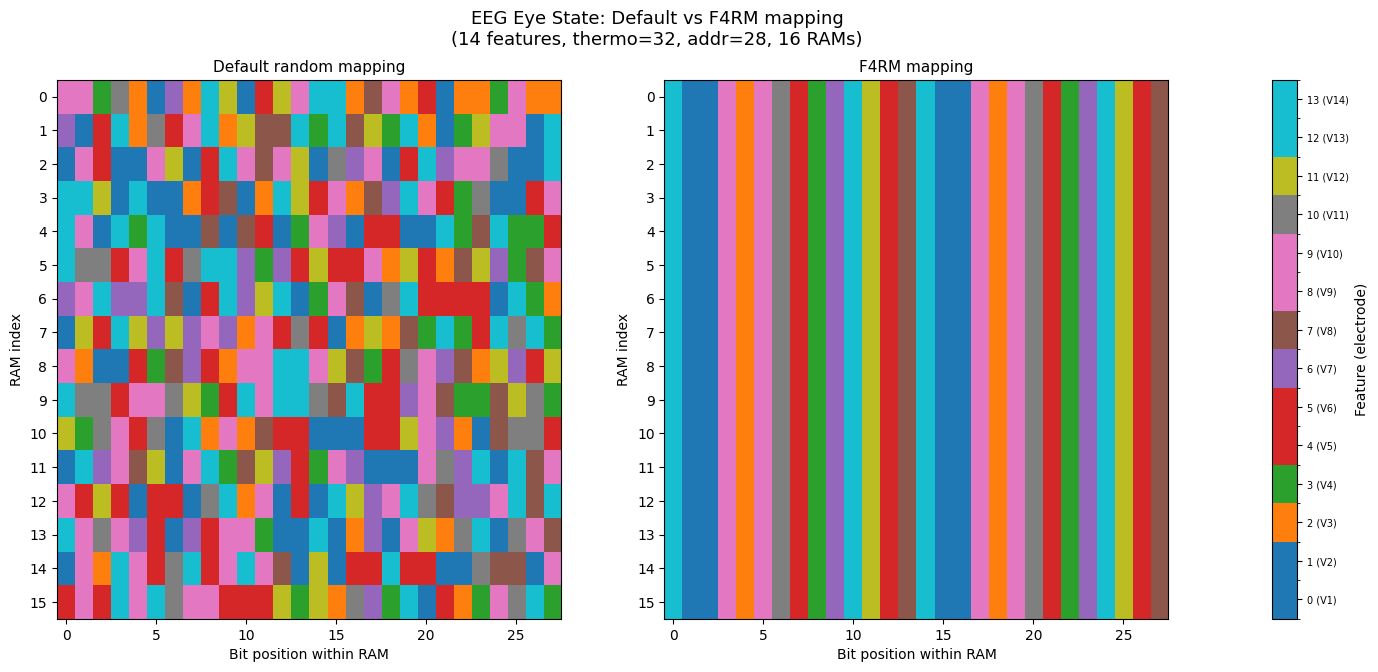
\includegraphics[width=0.75\linewidth]{figures/mapping_eeg.png}
  \caption{F4RM versus default random mapping on EEG Eye State ($n=14$ features, $a=28$, ratio $a/n=2.0$), visualized as bit-to-RAM assignment heatmaps. Each row is a RAM; each column is a bit position within the RAM; color encodes which feature the bit originates from. F4RM produces clean vertical stripes where each feature appears at consistent positions across all RAMs, while random mapping produces a chaotic pattern with visible same-feature clusters within individual rows.}
  \label{fig:mapping-comparison}
\end{figure}

\subsection{When F4RM Helps: A Testable Prediction}
\label{sec:testable-prediction}

Beyond the collision rate governed by $a/n$, a secondary factor is overall model capacity: if representational budget is abundant, wasted address slots matter less. F4RM's contribution should therefore be largest when (i) $a/n$ makes collisions frequent, and (ii) capacity is constrained. Thermometer size $t$ tests the second factor---increasing $t$ with $a, n$ fixed raises capacity without changing collision rate. Sweeping $t$ from $4$ to $512$ on four datasets (EEG Eye State, Magic Gamma, Yeast, Banknote), the F4RM$-$Random delta decays monotonically as $t$ grows (EEG: $+5.73$pp at $t=4$ to $+2.39$pp at $t=512$; Yeast: $+4.68$pp to $+0.81$pp). F4RM remains ahead throughout, but the decay confirms it improves information efficiency rather than adding capacity. This motivates the hyperparameter rule below.

\subsection{Address Size Selection}
\label{sec:address-size}

WiSARD's behavior depends strongly on the address size $a$, and the choice of $a$ has an established trade-off. Too small, and each RAM captures too narrow a bit pattern to support useful discrimination---the model under-fits. Too large, and the nominal address space $2^a$ exceeds what the training set can populate---most addresses remain empty, and the RAMs memorize training samples rather than generalize~\cite{susskind2022bthowen}. The standard approach in WiSARD work is per-dataset hyperparameter sweep~\cite{susskind2022bthowen}, in which $a$ and $t$ are tuned jointly on a validation set to maximize accuracy.

Sweeps confound a structural comparison of mappings: selecting hyperparameters per-mapping risks attributing to the mapping what is really a selection effect. To evaluate F4RM against random mapping fairly, we adopt a principled default rule and apply it identically to both:
\begin{equation}
a = \min\bigl(2n,\ \lfloor \log_2 m \rfloor\bigr),
\label{eq:addr-rule}
\end{equation}
where $n$ is the number of features and $m$ is the number of training samples. Thermometer size is fixed at $t = 8$ for all datasets.

Each term has an independent justification. The $2n$ term places $a/n = 2$, within the regime where same-feature collisions are frequent---not chosen to favor F4RM but to place both methods in a regime where any mapping-level difference is measurable. The $\lfloor \log_2 m \rfloor$ term caps the address space below the training set size; when $2^a > m$, most addresses are unreachable and RAMs tend to memorize samples rather than generalize. The minimum takes whichever bound binds: on small-sample datasets (Iris with $m=120$, Wine with $m=142$) the sample bound dominates, while on small-feature datasets (Haberman with $n=3$, Banknote with $n=4$) the feature bound does.

This rule is not intended to maximize per-dataset accuracy, and it does not: grid search yields higher peaks. Its purpose is to let F4RM's contribution be evaluated without confounding it with hyperparameter selection. The claim is not that F4RM achieves the highest possible accuracy but that, at identical hyperparameters chosen independently of the mapping, F4RM beats random mapping significantly on most datasets---and the default rule is what makes this claim rigorous.

Table~\ref{tab:configs} reports the address size, total bits, and number of RAMs produced by this rule for each dataset in our evaluation.

\begin{table}[!tbp]
  \centering
  \caption{Per-dataset hyperparameters produced by the rule $a = \min(2n, \lfloor \log_2 m \rfloor)$ with fixed $t = 8$, where $m$ is the number of training samples (80\% of the full dataset). Columns: total samples in the dataset, number of features $n$, address size $a$, address-to-feature ratio, total input bits $n \cdot t$, and number of RAMs per discriminator $R = \lceil n \cdot t / a \rceil$.}
  \label{tab:configs}
  \scriptsize
  \setlength{\tabcolsep}{3pt}
  \begin{tabular}{lrrrrrr}
    \toprule
    Dataset & Samples & $n$ & $a$ & $a/n$ & Bits & RAMs \\
    \midrule
    Iris                 & 150   & 4  & 6  & 1.50 & 32  & 6 \\
    Wine                 & 178   & 13 & 7  & 0.54 & 104 & 15 \\
    Seeds                & 210   & 7  & 7  & 1.00 & 56  & 8 \\
    Glass                & 214   & 9  & 7  & 0.78 & 72  & 11 \\
    Haberman             & 306   & 3  & 6  & 2.00 & 24  & 4 \\
    Ecoli                & 336   & 7  & 8  & 1.14 & 56  & 7 \\
    Ionosphere           & 351   & 34 & 8  & 0.24 & 272 & 34 \\
    Breast Cancer        & 569   & 30 & 8  & 0.27 & 240 & 30 \\
    Balance Scale        & 625   & 4  & 8  & 2.00 & 32  & 4 \\
    Pima Diabetes        & 768   & 8  & 9  & 1.12 & 64  & 8 \\
    Vehicle              & 846   & 18 & 9  & 0.50 & 144 & 16 \\
    Banknote             & 1372  & 4  & 8  & 2.00 & 32  & 4 \\
    Yeast                & 1484  & 8  & 10 & 1.25 & 64  & 7 \\
    Steel Plates         & 1941  & 33 & 10 & 0.30 & 264 & 27 \\
    Segment              & 2310  & 19 & 10 & 0.53 & 152 & 16 \\
    Waveform             & 5000  & 40 & 11 & 0.28 & 320 & 30 \\
    SatImage             & 6430  & 36 & 12 & 0.33 & 288 & 24 \\
    Pendigits            & 10992 & 16 & 13 & 0.81 & 128 & 10 \\
    EEG Eye State        & 14980 & 14 & 13 & 0.93 & 112 & 9 \\
    Magic Gamma          & 19020 & 10 & 13 & 1.30 & 80  & 7 \\
    Letter Recognition   & 20000 & 16 & 13 & 0.81 & 128 & 10 \\
    \bottomrule
  \end{tabular}
\end{table}


\section{F4RMS: F4RM enSemble}
\label{sec:f4rms}

We motivate the ensemble (Section~\ref{sec:f4rms-motivation}), justify sum-of-responses aggregation (Section~\ref{sec:f4rms-aggregation}), and consolidate the classifier (Section~\ref{sec:f4rms-classifier}).

\subsection{Motivation and Design}
\label{sec:f4rms-motivation}

F4RM replaces a randomized mapping with a constrained one, but the construction retains randomness along two axes: feature visit order and thermometer-level placement (Section~\ref{sec:f4rm-rule}). Different seeds therefore produce different valid F4RM mappings, all satisfying the rule but differing in which feature occupies which RAM position. This suggests an ensemble: train $K$ F4RM WiSARDs under different mapping seeds and aggregate their outputs. We call this \textbf{F4RMS} (F4RM enSemble).

Every F4RMS member is a \emph{full-feature} F4RM WiSARD: each reads every input feature, and members differ only in bit-to-RAM assignment. Ensembling WiSARDs is itself established practice---ULEEN~\cite{susskind2023uleen} combines multiple WiSARDs with different random permutations and reports consistent gains. F4RMS inherits this principle and substitutes F4RM mappings for purely random ones, so every member is individually stronger before aggregation.

An alternative would follow the Random Subspace Method~\cite{ho1998random}, giving each member a feature subset. We tested this and found it consistently weaker (details deferred to Section~\ref{sec:related-ensemble}): subspace ensembles trade member strength for decorrelation~\cite{breiman2001random}, a trade that loses for WiSARD members unable to reconstruct missing features.

\subsection{Aggregation}
\label{sec:f4rms-aggregation}

The second design choice is how to aggregate the members' outputs. WiSARD's discriminators produce a per-class response vector $\mathbf{r}^{(k)} \in \mathbb{R}^M$ for each ensemble member $k$, where $r^{(k)}_c$ is the summed RAM counter returned by member $k$'s discriminator for class $c$. Two natural aggregation options are majority voting---each member predicts a class, and the ensemble predicts the modal vote---and \textbf{sum-of-responses}: sum the $K$ response vectors element-wise and predict the class with the largest total:
\begin{equation}
\hat{y} = \arg\max_c \sum_{k=1}^{K} r^{(k)}_c.
\label{eq:sum-of-responses}
\end{equation}

We adopt sum-of-responses. Majority voting discards information: a confident correct prediction and a near-indifferent one both count as one vote, and a confidently wrong member is not penalized. Summing responses preserves magnitude, letting confident members contribute more. This is also the aggregation used by ULEEN~\cite{susskind2023uleen}, and it outperformed majority voting in our own design experiments.

\subsection{The F4RMS Classifier}
\label{sec:f4rms-classifier}

F4RMS with $K$ members trains $K$ independent F4RM WiSARDs with different mapping seeds at identical $a$ and $t$, aggregating their response vectors at inference. The only new hyperparameter is $K$.

F4RMS's cost scales linearly with $K$. Training is trivially parallel, so on parallel hardware inference latency matches single F4RM while raw compute grows linearly. F4RMS is therefore a parameter-free way to trade training time for accuracy at no deployment latency penalty. Section~\ref{sec:results} reports F4RMS at representative $K$.


\section{Experimental Methodology}
\label{sec:methodology}

We describe datasets (Section~\ref{sec:datasets}), the paired evaluation protocol (Section~\ref{sec:protocol}), and baselines, statistics, and environment (Section~\ref{sec:baselines-stats}).

\subsection{Datasets}
\label{sec:datasets}

We evaluate F4RM and F4RMS on 21 tabular classification datasets with 3 to 40 real-valued features, drawn from UCI and scikit-learn. Sample sizes range from 150 (Iris) to 20{,}000 (Letter Recognition) and class counts from 2 to 26. We selected standard benchmarks from the WNN literature~\cite{susskind2022bthowen,susskind2023uleen} and supplemented them with additional UCI datasets to broaden coverage. Table~\ref{tab:configs} lists per-dataset hyperparameters.

\subsection{Evaluation Protocol}
\label{sec:protocol}

For each dataset, we perform 200 independent evaluations. Each evaluation uses a stratified 80/20 train/test split seeded independently per evaluation; preprocessing applies min-max scaling and distributive thermometer thresholds~\cite{lima2020distributive} fit on the training fold only, with $t = 8$; all three methods (Random-mapped WiSARD, F4RM WiSARD, F4RMS with $K \in \{K_1, K_2, \ldots\}$) are trained and evaluated on the same split at the same address size $a$ from Section~\ref{sec:address-size}; per-method accuracy, training wall-clock time, and per-sample inference wall-clock time are recorded.

Pairing all methods on the same split within each evaluation enables paired statistical tests and removes split-induced variance from method-level comparisons. Across the 200 evaluations, the 200 split seeds are fixed and shared across datasets, so any dataset-level difference in variance is attributable to the dataset rather than split sampling. F4RM and F4RMS members use mapping seeds derived from the evaluation index, ensuring independent mapping draws across evaluations.

\subsection{Baselines, Statistics, and Environment}
\label{sec:baselines-stats}

The Random-mapping baseline is the standard WiSARD formulation: uniformly random bit-to-RAM assignment. Bleaching is enabled by default for all methods, matching the standard WiSARD implementation in \texttt{wisardpkg}~\cite{wisardpkg}, the reference Python library we use. F4RM and F4RMS are implemented on top of \texttt{wisardpkg} by supplying an explicit mapping computed by Algorithm~\ref{alg:f4rm} at model initialization. All code is available at \url{ANONYMIZED_REPO_URL}. The primary evaluation metric is top-1 classification accuracy on the held-out test fold, consistent with prior WiSARD tabular-classification work~\cite{susskind2022bthowen,susskind2023uleen}; all reported numbers, deltas, and statistical tests operate on this metric.

For each dataset, we compute the per-evaluation delta between each pair of methods (F4RM $-$ Random, F4RMS $-$ Random, F4RMS $-$ F4RM). For each pair-delta we report the mean, the Wilcoxon signed-rank test~\cite{wilcoxon1945individual} $p$-value, and a 95\% normal-approximation confidence interval on the mean paired delta ($\bar{\Delta} \pm 1.96\,\sigma_{\Delta}/\sqrt{n}$, with $n = 200$); every pair reported as significant at the Bonferroni-corrected threshold has a CI that excludes zero. The Wilcoxon test is preferred over the paired $t$-test because accuracy is bounded in $[0,1]$ and the delta distribution is rarely Gaussian. We apply Bonferroni correction with family-wise threshold $\alpha = 0.05 / 21 \approx 0.0024$ across the 21 datasets, and report a comparison as \emph{significant} only when the corrected threshold is met. All experiments ran on an Apple M4 Pro workstation (24 GB RAM, Python 3.13, CPU only); full replication of the 21-dataset evaluation takes approximately one hour.


\section{Results}
\label{sec:results}

We present F4RM vs Random (Section~\ref{sec:results-f4rm}), show how F4RMS compounds the benefit (Section~\ref{sec:results-f4rms}), and report costs (Section~\ref{sec:results-cost}).

\begin{table}[!tbp]
  \centering
  \caption{Main experimental results: Random, F4RM, and F4RMS at the best $K$ per dataset (F4RMS$^*$). Accuracies are mean $\pm$ standard deviation over 200 paired stratified 80/20 splits. Significance columns indicate whether the per-pair paired Wilcoxon p-value is below the Bonferroni-corrected threshold $\alpha = 0.05/21 \approx 0.0024$. A dash (---) indicates the comparison is not significant; a check ($\checkmark$) indicates significance. Best accuracy per dataset is bolded. Datasets are sorted by training-set size.}
  \label{tab:main-results}
  \setlength{\tabcolsep}{3pt}
  \scriptsize
  \resizebox{\textwidth}{!}{%
  \begin{tabular}{lrrrrllrrr}
    \toprule
    Dataset & $m$ & $n$ & $a$ & $K^*$ & Random & F4RM & F4RMS$^*$ & F4RM$>$R & F4RMS$>$R \\
    \midrule
    Iris               & 150   & 4  & 6  & 50 & 0.9503$\pm$0.037 & 0.9542$\pm$0.034 & \textbf{0.9602$\pm$0.034} & ---         & $\checkmark$ \\
    Wine               & 178   & 13 & 7  & 50 & 0.9665$\pm$0.029 & 0.9694$\pm$0.026 & \textbf{0.9792$\pm$0.021} & ---         & $\checkmark$ \\
    Seeds              & 210   & 7  & 7  & 10 & 0.9012$\pm$0.044 & 0.9043$\pm$0.042 & \textbf{0.9112$\pm$0.041} & ---         & $\checkmark$ \\
    Glass              & 214   & 9  & 7  & 25 & 0.6995$\pm$0.060 & 0.7077$\pm$0.058 & \textbf{0.7350$\pm$0.056} & ---         & $\checkmark$ \\
    Haberman           & 306   & 3  & 6  & 25 & 0.7147$\pm$0.044 & 0.7175$\pm$0.043 & \textbf{0.7212$\pm$0.034} & ---         & ---         \\
    Ecoli              & 336   & 7  & 8  & 50 & 0.8358$\pm$0.038 & 0.8447$\pm$0.038 & \textbf{0.8639$\pm$0.034} & $\checkmark$ & $\checkmark$ \\
    Ionosphere         & 351   & 34 & 8  & 50 & 0.9159$\pm$0.031 & 0.9106$\pm$0.031 & \textbf{0.9392$\pm$0.026} & ---         & $\checkmark$ \\
    Breast Cancer      & 569   & 30 & 8  & 25 & 0.9575$\pm$0.018 & 0.9600$\pm$0.017 & \textbf{0.9655$\pm$0.016} & ---         & $\checkmark$ \\
    Balance Scale      & 625   & 4  & 8  & 50 & 0.8202$\pm$0.030 & 0.8370$\pm$0.026 & \textbf{0.8711$\pm$0.020} & $\checkmark$ & $\checkmark$ \\
    Pima Diabetes      & 768   & 8  & 9  & 50 & 0.7065$\pm$0.032 & 0.7238$\pm$0.033 & \textbf{0.7462$\pm$0.030} & $\checkmark$ & $\checkmark$ \\
    Vehicle            & 846   & 18 & 9  & 50 & 0.6970$\pm$0.031 & 0.7075$\pm$0.031 & \textbf{0.7241$\pm$0.029} & $\checkmark$ & $\checkmark$ \\
    Banknote           & 1372  & 4  & 8  & 25 & 0.9800$\pm$0.011 & 0.9870$\pm$0.009 & \textbf{0.9955$\pm$0.004} & $\checkmark$ & $\checkmark$ \\
    Yeast              & 1484  & 8  & 10 & 50 & 0.4973$\pm$0.031 & 0.5426$\pm$0.028 & \textbf{0.5932$\pm$0.026} & $\checkmark$ & $\checkmark$ \\
    Steel Plates       & 1941  & 33 & 10 & 50 & 0.9136$\pm$0.021 & 0.9286$\pm$0.018 & \textbf{0.9693$\pm$0.009} & $\checkmark$ & $\checkmark$ \\
    Segment            & 2310  & 19 & 10 & 50 & 0.9414$\pm$0.011 & 0.9463$\pm$0.011 & \textbf{0.9593$\pm$0.009} & $\checkmark$ & $\checkmark$ \\
    Waveform           & 5000  & 40 & 11 & 50 & 0.7803$\pm$0.013 & 0.7909$\pm$0.012 & \textbf{0.8477$\pm$0.011} & $\checkmark$ & $\checkmark$ \\
    SatImage           & 6430  & 36 & 12 & 50 & 0.8658$\pm$0.009 & 0.8759$\pm$0.008 & \textbf{0.8947$\pm$0.007} & $\checkmark$ & $\checkmark$ \\
    Pendigits          & 10992 & 16 & 13 & 50 & 0.9756$\pm$0.004 & 0.9800$\pm$0.003 & \textbf{0.9874$\pm$0.002} & $\checkmark$ & $\checkmark$ \\
    EEG Eye State      & 14980 & 14 & 13 & 50 & 0.7407$\pm$0.013 & 0.8050$\pm$0.008 & \textbf{0.8931$\pm$0.006} & $\checkmark$ & $\checkmark$ \\
    Magic Gamma        & 19020 & 10 & 13 & 50 & 0.7800$\pm$0.014 & 0.8225$\pm$0.007 & \textbf{0.8630$\pm$0.005} & $\checkmark$ & $\checkmark$ \\
    Letter Recognition & 20000 & 16 & 13 & 50 & 0.8634$\pm$0.006 & 0.8886$\pm$0.006 & \textbf{0.9378$\pm$0.004} & $\checkmark$ & $\checkmark$ \\
    \midrule
    \multicolumn{5}{l}{\textbf{Significant (Bonferroni):}} & & & & 14/21 & 20/21 \\
    \bottomrule
  \end{tabular}%
  }
\end{table}

\subsection{F4RM vs Random Mapping}
\label{sec:results-f4rm}

Table~\ref{tab:main-results} reports the main result: on 21 tabular classification datasets, with 200 paired evaluations per dataset and Bonferroni correction at $\alpha = 0.05/21 \approx 0.0024$, F4RM beats random mapping on \textbf{14 of 21 datasets} with statistical significance, and never loses significantly. Across all datasets the mean per-evaluation delta is $+1.52$pp; the median is $+0.81$pp.

The datasets where F4RM's advantage is largest share a property the mechanism of Section~\ref{sec:f4rm-rule} predicts should matter: each feature carries meaningful, largely non-redundant signal. EEG Eye State ($+6.43$pp) has 14 electrode readings capturing distinct brain-activity channels; Yeast ($+4.53$pp) has 8 biological measurements curated for independent informativeness. Magic Gamma ($+4.25$pp), Letter Recognition ($+2.52$pp), Pendigits ($+0.44$pp), and SatImage ($+1.01$pp) all share moderate feature counts ($n$ between 8 and 36) with each feature contributing distinct information. On these, F4RM's guarantee that every RAM reads from every feature is exactly the right constraint: it prevents the model from accidentally leaving signal on the table.

The datasets where F4RM's advantage is small tell the complementary story. Ionosphere ($-0.54$pp, n.s.) and Breast Cancer ($+0.25$pp, n.s.) both have feature sets with heavy internal redundancy: Ionosphere's 34 features are complex-valued pairs from 17 pulse numbers~\cite{sigillito1989classification}, and Breast Cancer's 30 are mean/standard-error/``worst'' variants of 10 underlying measurements~\cite{street1993nuclear}. When omitted signal is carried by a neighboring feature, F4RM's coverage guarantee has little to redistribute.

This pattern defines three data regimes: a \emph{dense-signal regime} (EEG, Magic Gamma, Yeast, Letter Recognition, Pendigits, SatImage, Waveform, Vehicle, Segment) where each feature carries distinct information and F4RM delivers its largest gains; a \emph{redundant-feature regime} (Ionosphere, Breast Cancer) where correlated features make omissions cheap; and a \emph{small-sample regime} (Iris, Wine, Seeds, Glass, Haberman) where the $\lfloor \log_2 m \rfloor$ cap forces a small address size and run-to-run variance swamps sub-percentage-point effects---F4RM never significantly hurts here, and mean delta is positive on all five ($+0.38$, $+0.29$, $+0.31$, $+0.81$, $+0.28$ pp respectively). F4RM's contribution is to redistribute feature information evenly across RAMs; that redistribution is most valuable exactly when every feature carries signal worth redistributing.

\subsection{F4RMS Compounds the Benefit}
\label{sec:results-f4rms}

Table~\ref{tab:main-results} reports F4RMS at the per-dataset optimal $K^* \in \{10, 25, 50\}$. With this selection, \textbf{F4RMS beats random mapping on 20 of 21 datasets} with statistical significance and \textbf{beats single F4RM on 19 of 21}. The only dataset where F4RMS does not significantly improve over random mapping is Haberman; the two where F4RMS does not significantly exceed single F4RM are Haberman and Iris, both small enough ($m = 306$ and $m = 150$) that 200-run paired evaluation struggles to resolve small deltas after Bonferroni correction.

The compounding effect is most pronounced where F4RM itself is already strong. On EEG Eye State, F4RM's $+6.43$pp gain becomes $+15.24$pp under F4RMS; on Yeast, $+4.53$pp becomes $+9.58$pp; on Waveform, $+1.06$pp becomes $+6.74$pp. The ensemble's mapping diversity multiplies the benefit that a single F4RM mapping already captures.

More strikingly, F4RMS recovers gains on datasets where single F4RM is neutral. On Ionosphere, where single F4RM showed a slight non-significant negative delta, F4RMS delivers $+2.32$pp: the ensemble compensates for feature redundancy by combining mapping-diverse members, each emphasizing a different informative/redundant split. Wine and Glass transition similarly from non-significant F4RM gains to significant F4RMS gains of $+1.26$pp and $+3.55$pp. This is F4RMS's practical appeal: it generalizes F4RM's benefit to datasets where a single mapping alone cannot extract it.

F4RMS accuracy rises steeply from $K=1$ to $K=10$ and plateaus thereafter; gains beyond $K=25$ are generally under $+0.5$pp. This gives practitioners a clear cost-accuracy trade-off: $K=10$ captures most of F4RMS's benefit at $10\times$ the single-model training cost.

\subsection{Cost Analysis}
\label{sec:results-cost}

All methods share the same architecture and differ only in the mapping, so per-model costs are essentially identical: Random and F4RM both train in $\sim$1.1--1.2ms and infer at $\sim$4.4--4.7ms per batch, within measurement noise. The F4RM construction (Algorithm~\ref{alg:f4rm}) is $O(n \cdot t)$ and runs once at initialization. F4RMS scales linearly with $K$ in raw compute ($\sim$11ms train / $\sim$57ms infer at $K=10$; $\sim$50$\times$ at $K=50$), but its parallel members incur no latency penalty on parallel hardware. A practitioner can replace random mapping with F4RM at zero measurable cost; F4RMS extends the benefit at linear-in-$K$ compute and no parallelized latency penalty.


\section{Limitations and Future Work}
\label{sec:limitations}

We discuss scope conditions (Section~\ref{sec:limitations-details}) and outline extensions (Section~\ref{sec:future-work}).

\subsection{Limitations}
\label{sec:limitations-details}

\paragraph{Scope of evaluation.} We evaluate F4RM on tabular classification with at most 40 real-valued features, not on image data. The restriction is theoretical: as Section~\ref{sec:testable-prediction} establishes, F4RM's benefit requires $a/n$ large enough for frequent same-feature collisions, and image configurations (e.g., MNIST at $a/n = 0.036$) fall well below that threshold. Raising $a$ high enough on high-feature datasets would require $a \gg \log_2 m$, pushing the model past the memorization wall that our rule (Section~\ref{sec:address-size}) avoids---so the two constraints are jointly infeasible at standard training-set sizes. Preliminary MNIST and CIFAR-10 experiments confirmed the prediction, with F4RM deltas in the run-to-run noise. F4RM is therefore positioned as a rule for tabular data with thermometer-encoded continuous features, not a general-purpose replacement for random mapping.

\paragraph{Ensemble cost.} F4RMS training cost scales linearly with $K$; it parallelizes cleanly, but sequential deployments pay the full factor. $K=10$ captures most of the benefit.

\paragraph{Default rule is not optimal.} The rule of Section~\ref{sec:address-size} is designed to be mapping-independent, not accuracy-maximizing. Practitioners who can run per-dataset grid search should do so.

\paragraph{Binarization assumptions.} F4RM's justification depends on the monotonic structure of thermometer encoding; it would need revisiting under alternative schemes such as hash-based or learned binarizations.

\subsection{Future Work}
\label{sec:future-work}

\paragraph{Spatially-aware mapping for image data.} A variant replacing feature identity with patch or spatial-region identity could recover F4RM's benefit on image data at the appropriate granularity.

\paragraph{Analytical bounds on the benefit.} A theoretical result relating expected F4RM gain to a measurable dataset property---inter-feature mutual information or effective feature-matrix rank---would let practitioners predict the gain without running the experiment.

\paragraph{Heterogeneous F4RMS.} Varying $(a, t)$ across ensemble members, in the spirit of~\cite{susskind2023uleen}, is a natural extension.

\paragraph{Hyperparameter scaling.} A dedicated study of how $(a, t, m)$ jointly determine WiSARD accuracy would inform hyperparameter selection under different data-scale constraints.


\section{Conclusion}
\label{sec:conclusion}

Four decades of WiSARD research have explored ensemble structure, memory layout, bleaching, learned parameters, and alternative storage backends while leaving the bit-to-RAM mapping---defaulted to a uniformly random permutation---essentially unexamined. We have shown that this default leaves measurable accuracy on the table whenever the input has exploitable structure, as thermometer-encoded continuous features do. F4RM eliminates same-feature redundancy at zero cost: no new parameters, no training or inference changes, no hyperparameters beyond standard WiSARD. Across 21 tabular classification datasets with 200 paired evaluations each and Bonferroni correction, F4RM beats random mapping on 14 datasets and never significantly loses; F4RMS extends this to 20 significant wins out of 21 and beats single F4RM on 19 of 21.

The broader observation is that any component partitioning structured input into independent processing units should be designed to maximize coverage and minimize within-unit redundancy. F4RM is one instance of this lens applied to weightless networks; we expect others to emerge as WiSARD continues to be refined for edge and low-resource settings.

\begin{credits}
\subsubsection{\ackname} The authors used Claude Opus 4.7 (Anthropic) as a research assistant for code development, experimental analysis, and manuscript preparation.

\subsubsection{\discintname}
The authors have no competing interests to declare that are relevant to the content of this article.
\end{credits}

\makeatletter
\renewcommand\@biblabel[1]{#1.}
\let\oldbibliography\thebibliography
\renewcommand{\thebibliography}[1]{%
  \oldbibliography{#1}%
  \footnotesize
  \setlength{\itemsep}{-1.3ex}%
  \setlength{\parsep}{0pt}%
}
\makeatother
\bibliographystyle{splncs04}
\enlargethispage{3\baselineskip}
{\footnotesize\bibliography{references}}

\end{document}
